\documentclass{article}

\usepackage[paper=a4paper,left=30mm,right=30mm,top=25mm,bottom=25mm]{geometry}
\usepackage{amsmath,amssymb,amsthm,mathtools}
\usepackage{graphicx}
\usepackage{comment}
\usepackage{microtype}
\usepackage[numbers]{natbib}
\setlength{\bibsep}{4pt}
\usepackage[colorlinks=true,linkcolor=blue,citecolor=blue,urlcolor=blue]{hyperref}

\newtheorem{theorem}{Theorem}[section]
\newtheorem{lemma}[theorem]{Lemma}
\newtheorem{proposition}[theorem]{Proposition}
\newtheorem{corollary}[theorem]{Corollary}
\newtheorem{remark}[theorem]{Remark}

\newcommand{\C}{\mathcal{C}}
\newcommand{\I}{[0,1]}
\newcommand{\R}{\mathbb{R}}
\newcommand{\Q}{\mathcal{Q}}
\newcommand{\de}{\,\mathrm{d}}
\newcommand{\Om}{\Omega_{\tau,\phi,\beta}}
\DeclareMathOperator{\sgn}{sgn}
\newcommand{\keywords}[1]{\par\medskip\noindent\textbf{Keywords:} #1}

\hypersetup{
  pdftitle={The exact region determined by Kendall's tau, Spearman's footrule and Blomqvist's beta},
  pdfauthor={Jacob Israel Orenday Lares and Marcus Rockel},
  pdfsubject={Exact attainable regions of bivariate copula concordance coefficients},
  pdfkeywords={copula, Kendall's tau, Spearman's footrule, Blomqvist's beta, attainable region}
}

\title{
	The exact region determined by Kendall's tau, Spearman's footrule and Blomqvist's beta
}
\author{%
  Jacob Israel Orenday Lares\textsuperscript{*}
  \and
  Marcus Rockel\textsuperscript{$\dagger$}
}
\date{July 2026}

\begin{document}

\maketitle
\begin{center}
  \small\textit{\textsuperscript{*}Corresponding author. \texttt{jacob.orenday@gmail.com}}\\[2mm]
  \small\textit{%
    \textsuperscript{$\dagger$}Department of Quantitative Finance,\\
    Institute for Economics, University of Freiburg,\\
    Rempartstr. 16, 79098 Freiburg, Germany,\\
    \texttt{marcus.rockel@finance.uni-freiburg.de}
  }
\end{center}

\begin{abstract}
We determine the exact region $\Omega_{\tau,\phi,\beta}\coloneqq \{(\tau(C),\phi(C),\beta(C)):C\in\mathcal{C}\}$ of possible joint values of Kendall's tau, Spearman's footrule and Blomqvist's beta over the class $\mathcal{C}$ of all bivariate copulas.
The region consists precisely of all triples $(t,p,b)$ satisfying $-1\le b\le 1$, $\frac{3}{16}(1+b)^2-\frac12\le p\le 1-\frac38(1-b)^2$ and $\frac43 p-\frac13\le t\le \frac23 p+\frac13$.
In other words, the known exact $(\phi,\beta)$- and $(\tau,\phi)$-regions already characterize the joint region, so that, once the value of Spearman's footrule is fixed, Blomqvist's beta imposes no additional sharp restriction on the possible values of Kendall's tau.
The proof is constructive: two one-parameter families of shuffles of $M$ realize the extreme values of Kendall's tau along the lower boundary of the $(\phi,\beta)$-region, ordinal sums spread these families through the whole region, and the vertical fibres are filled using the biaffinity of the concordance function.
We further show that $\Omega_{\tau,\phi,\beta}$ is convex with rectangular fixed-footrule sections, identify an affine symmetry of its fibres about $\tau=\phi$, and compute its volume, which equals $\frac{31}{40}$.
\end{abstract}

\keywords{Copula; Rank correlation; Concordance measure; Attainable region; Shuffle of $M$; Ordinal sum; Biaffine concordance function; Medial correlation coefficient}
\par\smallskip\noindent\textbf{MSC 2020:} 62H05; 62H20

\section{Introduction}\label{sec:intro}

Rank correlation coefficients are among the most widely used summaries of dependence between two random quantities, because they are invariant under strictly increasing transformations of either margin and require no moment assumptions.
In practice, several such coefficients are often estimated from the same data set, either to narrow down a suitable dependence model or to capture different aspects of association.
At the population level, a joint attainable region records exactly which coefficient vectors can arise from a common dependence structure.
%For the present triple, the central issue is whether the two known bivariate regions are jointly sufficient or whether an additional genuinely ternary constraint appears.
The study of exact regions goes back to the classical inequalities between Kendall's tau and Spearman's rho and has remained active ever since.
Here we settle the problem for Kendall's tau, Spearman's footrule and Blomqvist's beta, for which the answer takes a particularly simple form.

A (bivariate) \emph{copula} is a distribution function on $\I^2$ with uniform marginals; by Sklar's theorem, see \cite{sklar1959fonctions}, copulas couple multivariate distribution functions with their one-dimensional margins, and the copula is unique whenever the margins are continuous; see \cite{nelsen2006introduction,durante2016principles} for an overview.
We denote by $\C$ the class of all bivariate copulas, by $M(u,v)\coloneqq \min\{u,v\}$ the comonotonicity copula and by $W(u,v)\coloneqq \max\{0,u+v-1\}$ the countermonotonicity copula.
Measures of concordance, formalized axiomatically by Scarsini in \cite{scarsini1984measures}, summarize on the scale $[-1,1]$ the degree of positive dependence captured by a copula.
The most prominent of the three coefficients studied in this paper is Kendall's tau, introduced in \cite{kendall1938new}, which is the probability of concordance minus the probability of discordance of two independent copies of the underlying random vector and, in copula form, becomes
\begin{equation}\label{eq:tau-def}
\tau(C)\coloneqq 4\int_{\I^2} C(u,v)\de C(u,v)-1.
\end{equation}
Spearman's footrule, introduced in \cite{spearman1906footrule} as an easily computed companion to Spearman's rank correlation, averages absolute rank differences; in terms of the diagonal section $\delta_C(u)\coloneqq C(u,u)$ it can be written as
\begin{equation}\label{eq:phi-def}
\phi(C)\coloneqq 6\int_0^1 \delta_C(u)\de u-2.
\end{equation}
Blomqvist's beta, introduced in \cite{blomqvist1950measure} and also known as the medial correlation coefficient, compares the probability mass of the four quadrants determined by the medians and is given by
\begin{equation}\label{eq:beta-def}
\beta(C)\coloneqq 4C\bigl(\tfrac12,\tfrac12\bigr)-1.
\end{equation}
Kendall's tau and Blomqvist's beta are concordance measures in the sense of Scarsini, while Spearman's footrule is only a weak concordance measure with range $[-\frac12,1]$; see \cite{genest2010spearman} for a review of the footrule.

The exact form of the mutual constraints between such coefficients has received considerable attention.
Schreyer et al.\ determined the exact $(\tau,\rho)$-region for Spearman's rho $\rho$ in \cite{schreyer2017exact}, settling a long-standing open question.
The exact regions of Spearman's footrule and Gini's gamma $\gamma$ with respect to Blomqvist's beta were obtained in \cite{kokolbukovsek2021spearman}, the regions of Kendall's tau with respect to the footrule and to Gini's gamma in \cite{kokolbukovsek2023exact}, and the $(\tau,\beta)$-region in \cite[Thm.~5]{kokolbukovsek2019relation}.
Beyond feasibility, exact regions have also been used to quantify how strongly knowledge of one coefficient restricts another: the concordance similarity measure was introduced in \cite{kokolbukovsek2022exact} and subsequently applied to Kendall's tau in \cite[Sec.~5]{kokolbukovsek2023exact}.
Recently, the first exact regions determined by \emph{three} coefficients simultaneously have been described: the $(\beta,\phi,\gamma)$-region in \cite{kokolbukovsek2026exact} and the $(\phi,\gamma,\tau)$-region in \cite{kokolbukovsek2026footrule}.

In this paper we determine the exact region
\[
\Om\coloneqq \bigl\{(\tau(C),\phi(C),\beta(C)):C\in\C\bigr\}\subseteq\R^3.
\]
Throughout, we use the boundary functions
\begin{equation}\label{eq:boundary-functions}
L(b)\coloneqq \tfrac{3}{16}(1+b)^2-\tfrac12,\qquad
U(b)\coloneqq 1-\tfrac38(1-b)^2,\qquad
\ell(p)\coloneqq \tfrac43 p-\tfrac13,\qquad
u(p)\coloneqq \tfrac23 p+\tfrac13
\end{equation}
of the exact $(\phi,\beta)$-region \cite[Thm.~11]{kokolbukovsek2021spearman} and the exact $(\tau,\phi)$-region \cite[Thm.~4]{kokolbukovsek2023exact}.
The following theorem is our main result; Figure~\ref{fig:region} illustrates the region.

\begin{theorem}[Exact $(\tau,\phi,\beta)$-region]\label{thm:main}
A triple $(t,p,b)\in\R^3$ equals $(\tau(C),\phi(C),\beta(C))$ for some copula $C\in\C$ if and only if $-1\le b\le 1$, $L(b)\le p\le U(b)$ and $\ell(p)\le t\le u(p)$; that is,
\begin{equation}\label{eq:region}
\Om=\bigl\{(t,p,b)\in\R^3:\ -1\le b\le 1,\ L(b)\le p\le U(b),\ \ell(p)\le t\le u(p)\bigr\}.
\end{equation}
\end{theorem}

\begin{figure}[t!]
\centering
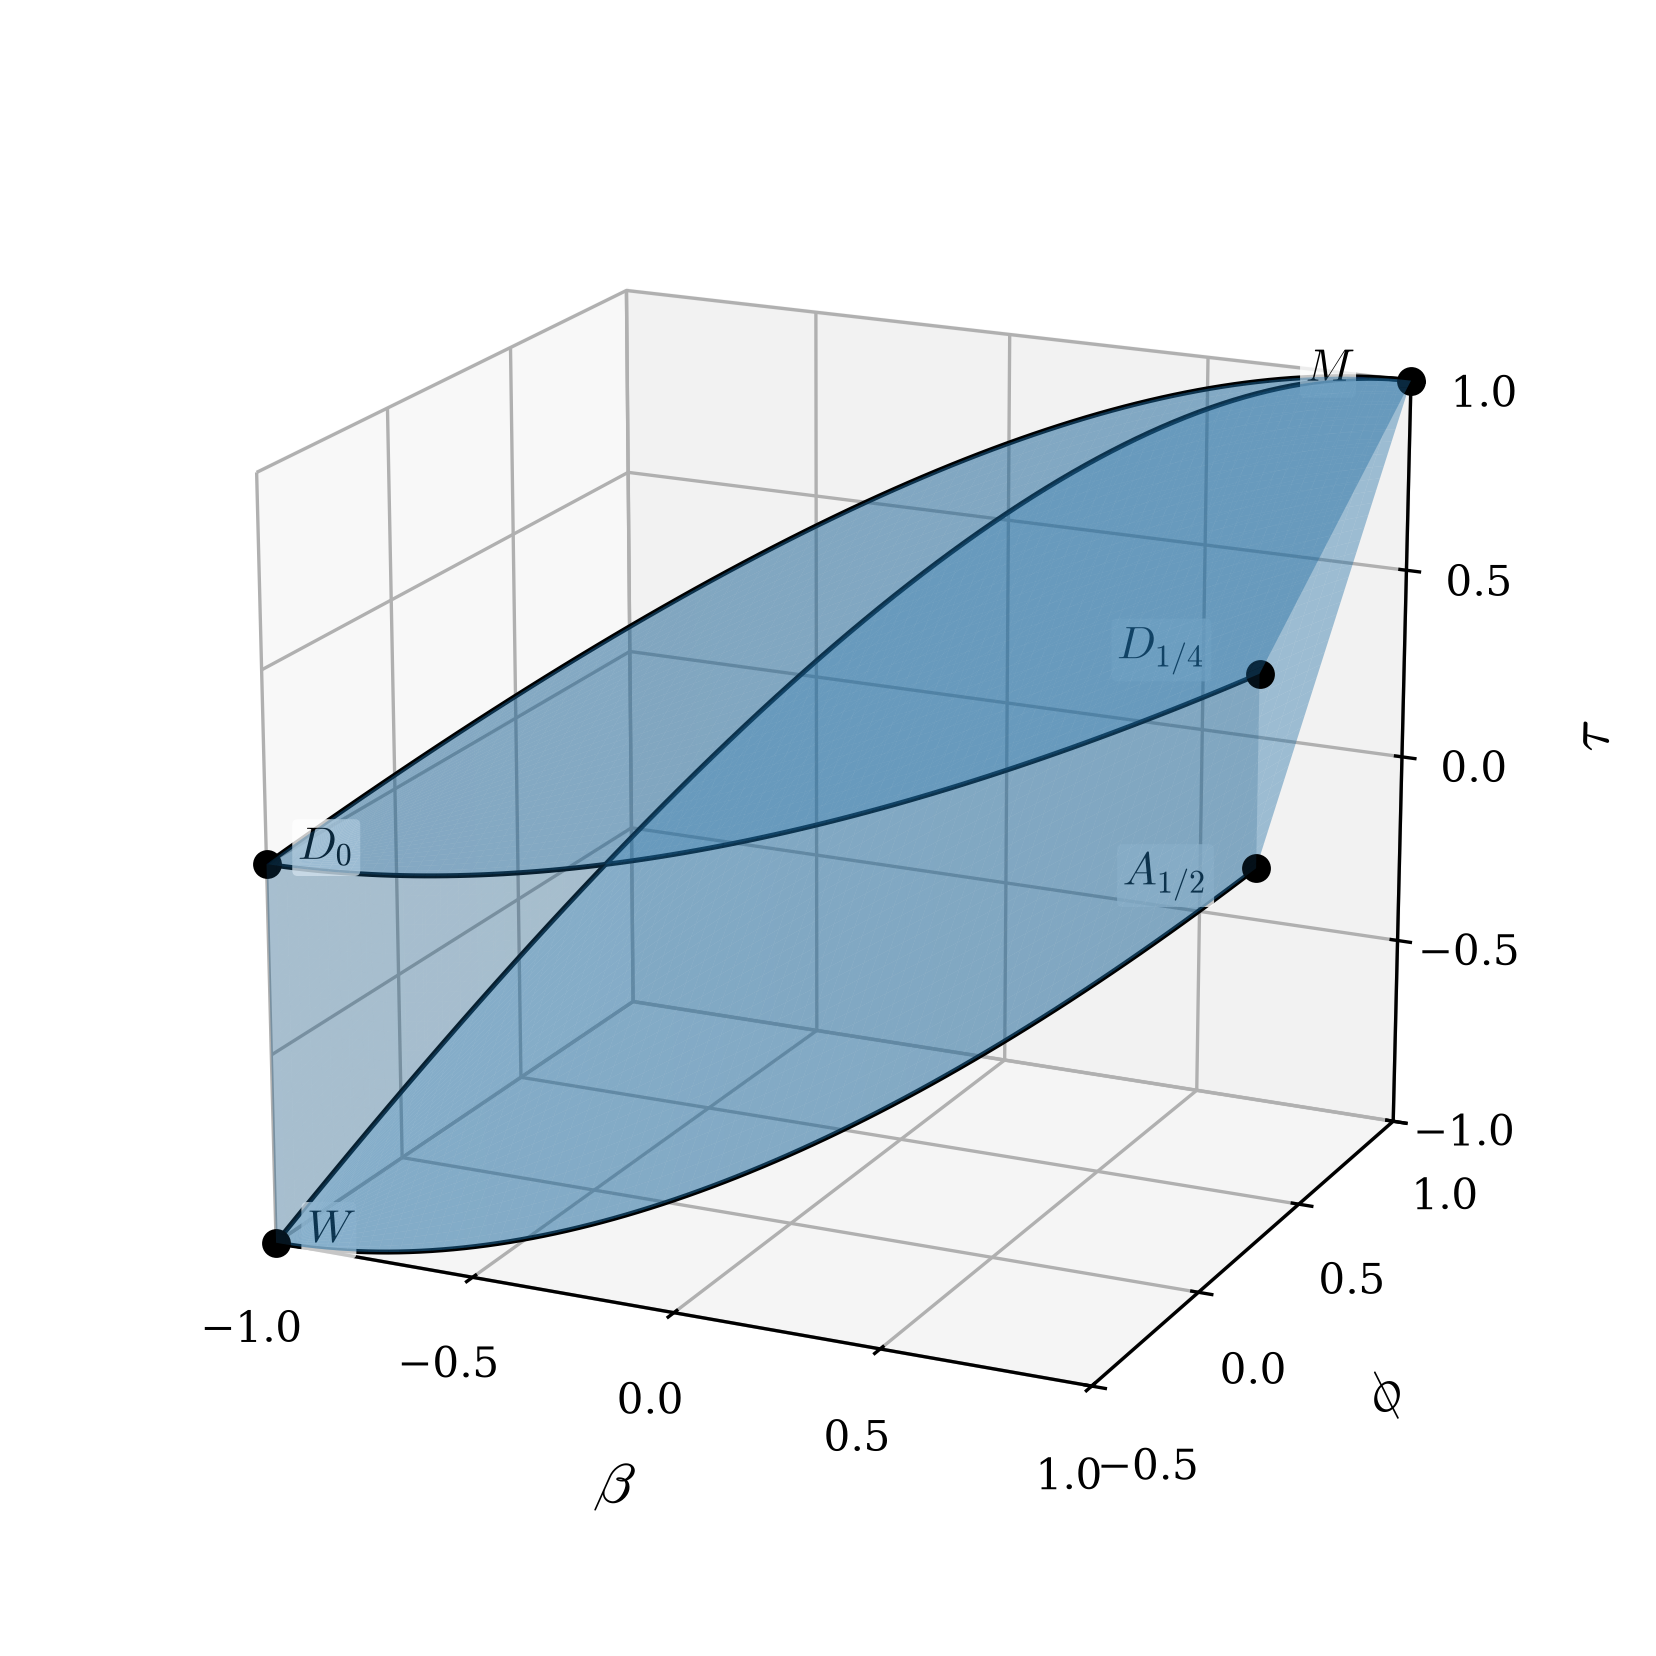
\includegraphics[width=0.72\textwidth]{images/region_beta_phi_tau.png}
\caption{
  The exact region $\Om$ from Theorem~\ref{thm:main}, plotted using \eqref{eq:region}.
  The lower and upper faces are the planes $t=\ell(p)=\frac43p-\frac13$ and $t=u(p)=\frac23p+\frac13$, and the side faces lie above the parabolas $p=L(b)$ and $p=U(b)$ that bound the $(\phi,\beta)$-region.
  For each admissible pair $(p,b)$, the vertical fibre is the interval $[\ell(p),u(p)]$ and has length $\frac23(1-p)$, independent of $b$.
  The labelled black dots mark the five corner points and the copulas that attain them.
  The families $A_r$ and $D_q$ from Section~\ref{sec:seeds} trace the edges $W$--$A_{1/2}$ and $D_0$--$D_{1/4}$, and the ordinal-sum families $B_{a,W}$ and $B_{a,D_0}$ trace the other two edges, $W$--$M$ and $D_0$--$M$, see Remark~\ref{rem:boundary-edges}.
}
\label{fig:region}
\end{figure}

The inclusion ``$\subseteq$'' in \eqref{eq:region} follows directly from the known bivariate regions (Proposition~\ref{prop:known} below).
Theorem~\ref{thm:main} shows that there is no further constraint: $\Om$ is exactly the intersection of the two cylinders over the $(\tau,\phi)$- and $(\phi,\beta)$-regions.
Equivalently, for every admissible pair $(p,b)$ the fibre $\{t:(t,p,b)\in\Om\}$ is the full interval $[\ell(p),u(p)]$, so that, given the value of Spearman's footrule, the value of Blomqvist's beta imposes no additional sharp restriction on Kendall's tau.
This purely bivariate constraint structure contrasts with the regions determined in \cite{kokolbukovsek2026exact,kokolbukovsek2026footrule}, whose boundaries contain faces described by genuinely ternary constraints.

The proof gives an explicit construction.
We first give two one-parameter families of shuffles of $M$ that attain the extreme values of Kendall's tau along the lower boundary $p=L(b)$ of the $(\phi,\beta)$-region; see Propositions~\ref{prop:lower-seed} and~\ref{prop:upper-seed} and Figures~\ref{fig:A-seeds} and~\ref{fig:D-seeds}.
Ordinal sums with $M$ then transport these families to every admissible pair $(p,b)$, the key observation being that $\tau$ and $\phi$ transform under such ordinal sums with the same quadratic factor while $\beta$ transforms linearly, see \eqref{eq:ordinal-sum} below.
Finally, $\tau(C)=\Q(C,C)$ for the biaffine concordance function $\Q$, while $\phi$ and $\beta$ are affine in the copula.
The intermediate value theorem applied to convex combinations then fills each vertical fibre.

The rest of the paper is organized as follows.
Section~\ref{sec:prelim} collects notation, the two known bivariate regions and the transformation behaviour of the three coefficients under ordinal sums.
In Section~\ref{sec:seeds} we construct the two shuffle families and compute their coefficient values by means of a closed formula for Kendall's tau of a shuffle of $M$ (Lemma~\ref{lem:shuffle-tau}).
Section~\ref{sec:proof} contains the proof of Theorem~\ref{thm:main}, the geometry of its fixed-footrule sections (Corollary~\ref{cor:fixed-phi}) and the resulting $(\tau,\beta)$-projection (Corollary~\ref{cor:beta-tau}), which recovers the region of \cite{kokolbukovsek2019relation}.
Section~\ref{sec:conclusion} closes with the volume of $\Om$ and some open problems.

\section{Preliminaries}\label{sec:prelim}

The set $\C$ is convex.
Throughout, an integral with respect to a copula denotes the Lebesgue--Stieltjes integral with respect to the probability measure induced by that copula.
For $C_1,C_2\in\C$, the \emph{concordance function} introduced by Kruskal in \cite{kruskal1958ordinal} is
\begin{equation}\label{eq:Q-def}
\Q(C_1,C_2)\coloneqq 4\int_{\I^2} C_2(u,v)\de C_1(u,v)-1,
\end{equation}
so that $\tau(C)=\Q(C,C)$ by \eqref{eq:tau-def}.
The function $\Q$ is symmetric in its two arguments, see \cite[Cor.~5.1.2]{nelsen2006introduction}.
It is affine in its second argument by linearity of the integral and in its first argument because a convex combination of copulas induces the same convex combination of their probability measures.

Our proof uses the following two known exact regions.

\begin{proposition}[Known bivariate regions]\label{prop:known}
Every copula $C\in\C$ satisfies
\begin{align}
\ell(\phi(C))&\le\tau(C)\le u(\phi(C)),\label{eq:ft-region}\\
L(\beta(C))&\le\phi(C)\le U(\beta(C)),\label{eq:bf-region}
\end{align}
with $L,U,\ell,u$ as in \eqref{eq:boundary-functions}, and both pairs of bounds are pointwise attained.
\end{proposition}

The $(\tau,\phi)$-region \eqref{eq:ft-region} was determined in \cite[Thm.~4]{kokolbukovsek2023exact} and is also collected in \cite[Prop.~2.1]{kokolbukovsek2026footrule}; the $(\phi,\beta)$-region \eqref{eq:bf-region} is given in \cite[Thm.~11]{kokolbukovsek2021spearman}, see also \cite[Thm.~7]{kokolbukovsek2019relation}.

A \emph{shuffle of $M$} in the sense of \cite{mikusinski1992shuffles} is a copula $C=M(n,J,\pi,\varepsilon)$ specified by a partition $J=(x_1,\dots,x_{n-1})$, $0=x_0\le x_1\le\dots\le x_n=1$, of $\I$ into $n$ strips of widths $s_i\coloneqq x_i-x_{i-1}$, a permutation $\pi$ of $\{1,\dots,n\}$ (written below in one-line notation) and a vector of signs $\varepsilon\in\{-1,1\}^n$.
Writing $0=y_0\le y_1\le\dots\le y_n=1$ for the partition of the second coordinate with band widths $y_k-y_{k-1}\coloneqq s_{\pi^{-1}(k)}$, the copula $M(n,J,\pi,\varepsilon)$ distributes mass $s_i$ uniformly on the diagonal (if $\varepsilon_i=1$) or the antidiagonal (if $\varepsilon_i=-1$) of the square $[x_{i-1},x_i]\times[y_{\pi(i)-1},y_{\pi(i)}]$, for $i=1,\dots,n$.
We allow zero strip widths in this definition, so that the endpoint cases used below are included as possibly degenerate shuffles of $M$; equivalently, they may be obtained by continuity from the corresponding nondegenerate shuffles.

For $a\in[0,\frac12]$ and $C\in\C$, let $B_{a,C}$ denote the ordinal sum of $\{C\}$ with respect to the single interval $(a,1-a)$, i.e., the copula that rescales $C$ to the central square $[a,1-a]^2$ and coincides with $M$ elsewhere on $\I^2$; for ordinal sums see \cite[Sec.~3.2.2]{nelsen2006introduction}.
Writing $\alpha\coloneqq 1-2a\in[0,1]$, the formulas of \cite[Lem.~3.8]{kokolbukovsek2026footrule} read
\begin{equation}\label{eq:ordinal-sum}
\tau(B_{a,C})=\alpha^2\tau(C)+1-\alpha^2,\qquad
\phi(B_{a,C})=\alpha^2\phi(C)+1-\alpha^2,\qquad
\beta(B_{a,C})=\alpha\,\beta(C)+1-\alpha.
\end{equation}
Here $\tau$ and $\phi$ transform by the same affine map $z\mapsto\alpha^2z+1-\alpha^2$, while $\beta$ has a linear factor.

\section{Two families of shuffles}\label{sec:seeds}

To prove Theorem~\ref{thm:main}, we need copulas that attain the extreme values $\ell(p)$ and $u(p)$ of Kendall's tau for a prescribed pair $(\phi,\beta)=(p,b)$ on the lower boundary $p=L(b)$ of the $(\phi,\beta)$-region.
We construct them as shuffles of $M$, shown in Figures~\ref{fig:A-seeds} and~\ref{fig:D-seeds}, and compute their Kendall's tau using the following formula.

\begin{lemma}[Kendall's tau of a shuffle of $M$]\label{lem:shuffle-tau}
Every shuffle of $M$, $C=M(n,J,\pi,\varepsilon)$, with strip widths $s_1,\dots,s_n$ satisfies
\begin{equation}\label{eq:shuffle-tau}
\tau(C)=\sum_{i=1}^n\varepsilon_i s_i^2
+2\sum_{1\le i<j\le n}\sgn\bigl(\pi(j)-\pi(i)\bigr)\,s_i s_j.
\end{equation}
\end{lemma}

\begin{proof}
Let $(X,Y)$ and $(X',Y')$ be independent random vectors with copula $C$.
Deleting zero-width strips and relabelling does not change either the copula or the right-hand side of \eqref{eq:shuffle-tau}, so we may assume that $s_i>0$ for every $i$.
By \cite[Sec.~5.1.1]{nelsen2006introduction},
\[
\tau(C)=\mathbb{P}\bigl((X-X')(Y-Y')>0\bigr)-\mathbb{P}\bigl((X-X')(Y-Y')<0\bigr).
\]
Both points fall into strip $i$ with probability $s_i^2$.
Given this event, they are almost surely concordant if $\varepsilon_i=1$ and almost surely discordant if $\varepsilon_i=-1$, giving the contribution $\varepsilon_i s_i^2$.
The two points fall into distinct strips $i<j$ with probability $2s_is_j$.
In this case they are concordant exactly when the vertical order of the bands agrees with the horizontal order of the strips, that is, when $\pi(i)<\pi(j)$, giving the contribution $2\sgn(\pi(j)-\pi(i))s_is_j$.
These events are exhaustive up to null sets, and summing the contributions proves \eqref{eq:shuffle-tau}.
\end{proof}

\begin{proposition}[Lower seed]\label{prop:lower-seed}
For $r\in[0,\frac12]$ let
\[
A_r\coloneqq M\Bigl(4,\bigl(\tfrac12-r,\tfrac12,\tfrac12+r\bigr),(4,2,3,1),(-1,-1,-1,-1)\Bigr).
\]
Then
\[
\bigl(\tau(A_r),\phi(A_r),\beta(A_r)\bigr)
=\bigl(\ell(L(4r-1)),\;L(4r-1),\;4r-1\bigr)
=\bigl(4r^2-1,\;3r^2-\tfrac12,\;4r-1\bigr).
\]
\end{proposition}

\begin{figure}[htbp!]
\centering
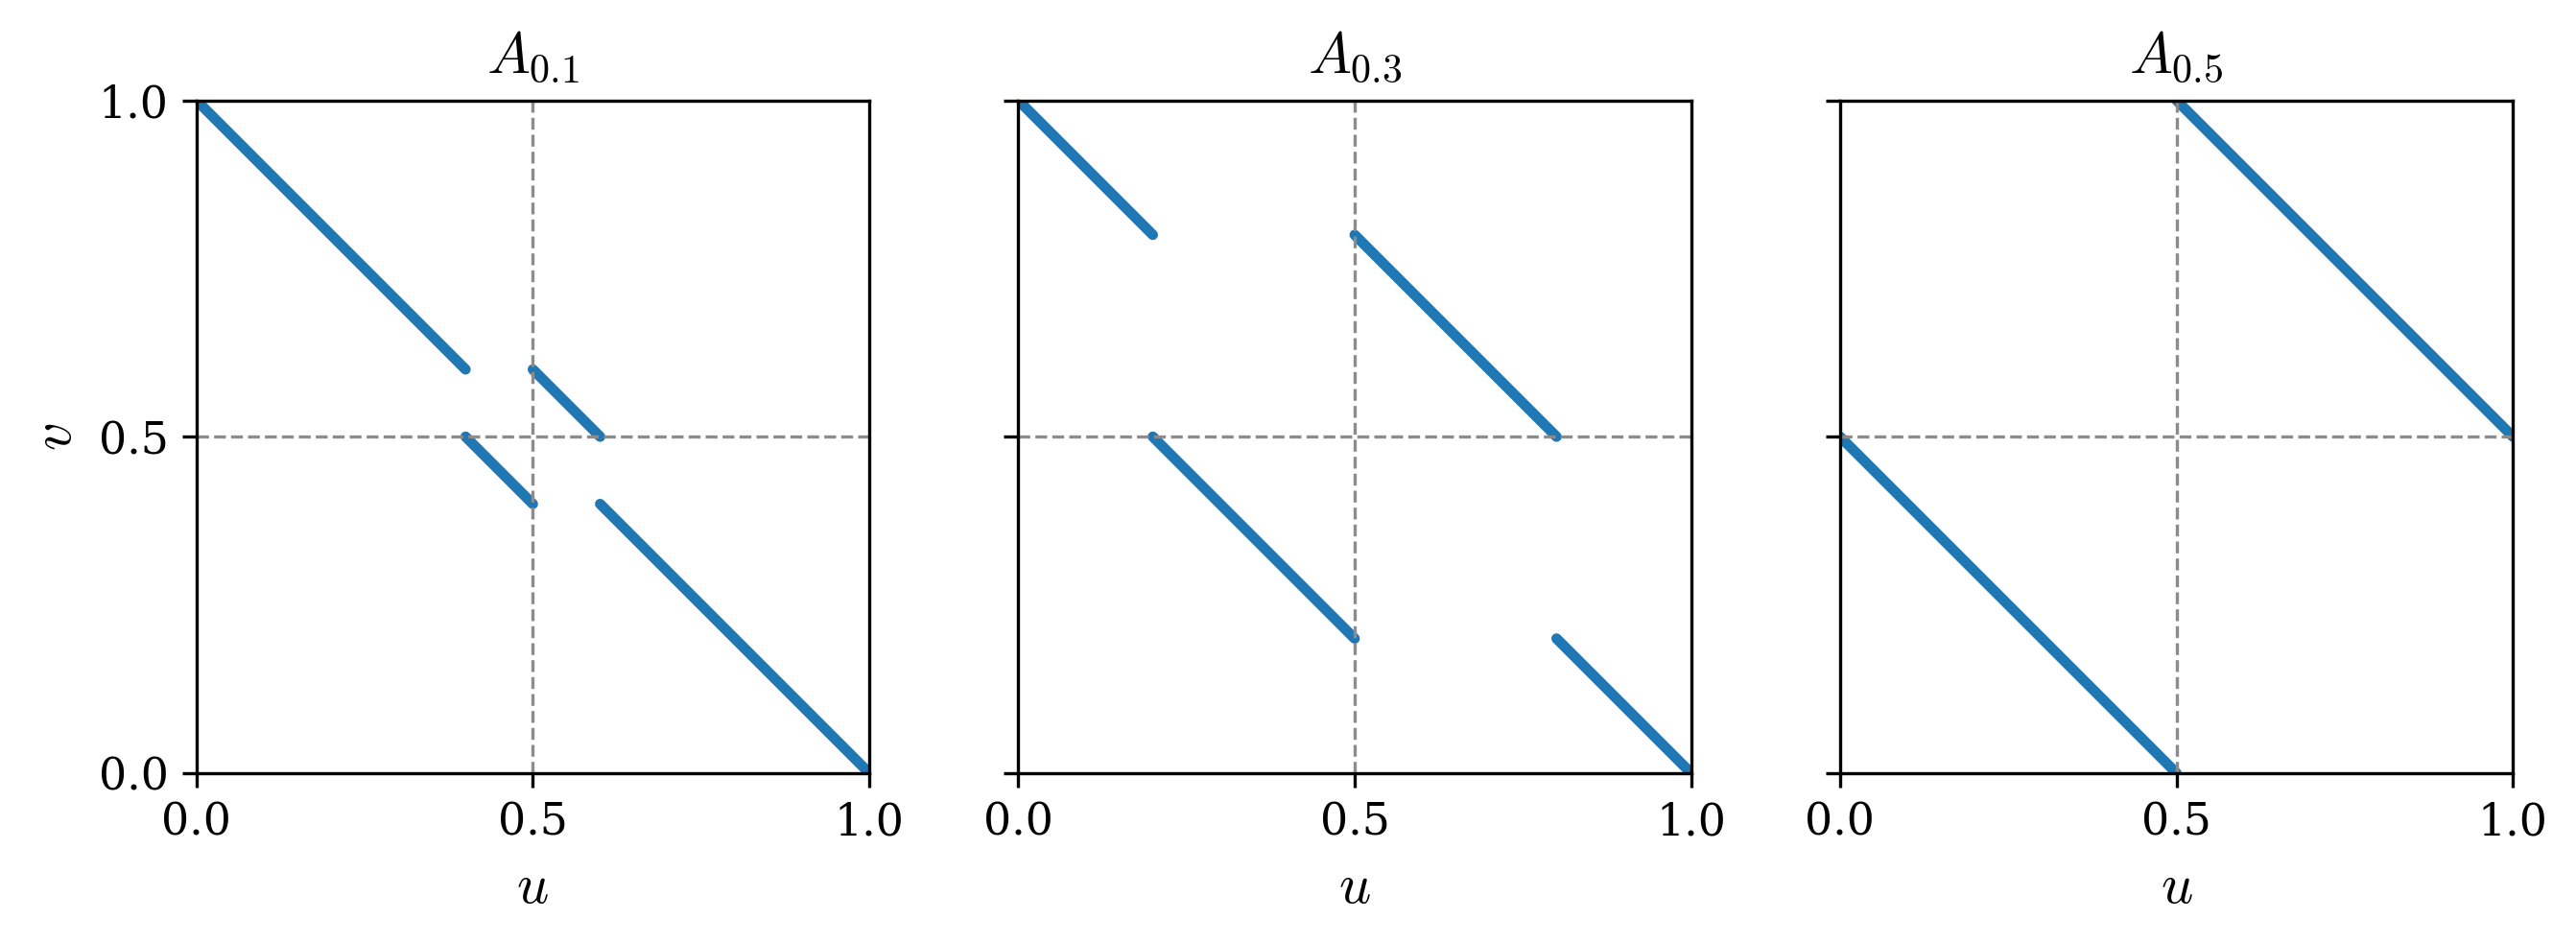
\includegraphics[width=0.95\textwidth]{images/A_seed_supports.png}
\caption{Supports of the lower seeds $A_r$ of Proposition~\ref{prop:lower-seed} for $r=0.1$, $0.3$ and $0.5$; dashed lines mark $u=\frac12$ and $v=\frac12$.
The copulas spread their mass uniformly on antidiagonal segments.
As $r$ increases, the two central segments lengthen while the two outer segments shrink, degenerating at $r=\frac12$.
The family traces the lower edge of $\Om$ above the boundary $\phi=L(\beta)$, with $(\tau,\phi,\beta)=(4r^2-1,3r^2-\frac12,4r-1)$.}
\label{fig:A-seeds}
\end{figure}

\begin{proof}
Write $a\coloneqq \frac12-r$, so that the strip widths of $A_r$ are $(a,r,r,a)$ and the band widths are likewise $(a,r,r,a)$.
The permutation $(4,2,3,1)$ maps the first strip to the top band $[\frac12+r,1]$ and the second strip, of width $r$, to the band $[a,\frac12]\subseteq[0,\frac12]$, so the mass in $[0,\frac12]^2$ equals $r$ and $\beta(A_r)=4r-1$ by \eqref{eq:beta-def}.
A direct computation of the diagonal section gives
\[
\delta_{A_r}(x)=
\begin{cases}
0, & 0\le x\le \frac12-\frac r2,\\
2x+r-1, & \frac12-\frac r2<x\le \frac12,\\
r, & \frac12<x\le \frac12+\frac r2,\\
2x-1, & \frac12+\frac r2<x\le 1,
\end{cases}
\]
so $\int_0^1\delta_{A_r}(x)\de x=\frac14+\frac{r^2}{2}$ and, by \eqref{eq:phi-def}, $\phi(A_r)=3r^2-\frac12=L(4r-1)$.
In Lemma~\ref{lem:shuffle-tau} the within-strip terms sum to $-2a^2-2r^2$ and the between-strip terms to $2(r^2-a^2-4ar)$, so
\[
\tau(A_r)=-4a^2-8ar=-4a(a+2r)=-4\bigl(\tfrac12-r\bigr)\bigl(\tfrac12+r\bigr)=4r^2-1,
\]
and indeed $\ell(3r^2-\frac12)=4r^2-1$.
\end{proof}

\begin{proposition}[Upper seed]\label{prop:upper-seed}
For $q\in[0,\frac14]$ let
\[
D_q\coloneqq M\Bigl(6,\bigl(q,\tfrac12-q,\tfrac12,\tfrac12+q,1-q\bigr),(3,5,1,6,2,4),(1,1,1,1,1,1)\Bigr).
\]
Then
\[
\bigl(\tau(D_q),\phi(D_q),\beta(D_q)\bigr)
=\bigl(u(L(8q-1)),\;L(8q-1),\;8q-1\bigr)
=\bigl(8q^2,\;12q^2-\tfrac12,\;8q-1\bigr).
\]
\end{proposition}

\begin{proof}
The strip widths of $D_q$ are $(q,a,q,q,a,q)$ with $a\coloneqq \frac12-2q$.
The three strips contained in $[0,\frac12]$ are mapped to the bands $[\frac12-q,\frac12]$, $[\frac12+q,1-q]$ and $[0,q]$, respectively, so the mass in $[0,\frac12]^2$ equals $2q$ and $\beta(D_q)=8q-1$ by \eqref{eq:beta-def}.

We next compute Spearman's footrule from the diagonal section.
If $(X,Y)$ has copula $D_q$, then $\delta_{D_q}(u)=\mathbb{P}(\max\{X,Y\}\le u)$, and Fubini's theorem gives $\int_0^1\delta_{D_q}(u)\de u=\mathbb{E}[1-\max\{X,Y\}]$.
Since all signs of $D_q$ are positive, $D_q$ is supported on the graph of the measure-preserving map
\[
h(x)=
\begin{cases}
x+\frac12-q, & 0\le x<q,\\
x+\frac12, & q\le x<\frac12-q,\\
x-\frac12+q, & \frac12-q\le x<\frac12,\\
x+\frac12-q, & \frac12\le x<\frac12+q,\\
x-\frac12, & \frac12+q\le x<1-q,\\
x-\frac12+q, & 1-q\le x\le1,
\end{cases}
\]
where formulas on a zero-length strip are immaterial.
Writing $I_i\coloneqq \int_{x_{i-1}}^{x_i}(1-\max\{x,h(x)\})\de x$ for the contribution of the $i$th strip, a direct stripwise integration gives
\[
I_1=I_3=\frac q2+\frac{q^2}{2},\qquad
I_2=I_5=\frac18-\frac q2,\qquad
I_4=I_6=\frac{q^2}{2},
\]
so that
\[
\int_0^1\delta_{D_q}(u)\de u=\sum_{i=1}^6 I_i=\frac14+2q^2
\qquad\text{and}\qquad
\phi(D_q)=6\Bigl(\frac14+2q^2\Bigr)-2=12q^2-\frac12
\]
by \eqref{eq:phi-def}.

Finally, Kendall's tau follows from Lemma~\ref{lem:shuffle-tau}: the within-strip terms sum to $4q^2+2a^2$, while the between-strip terms sum to $2(2q^2-a^2)$, so
\[
\tau(D_q)=4q^2+2a^2+2(2q^2-a^2)=8q^2.
\]
Thus $L(8q-1)=12q^2-\frac12=\phi(D_q)$ and $u(12q^2-\frac12)=8q^2=\tau(D_q)$.
\end{proof}

\begin{figure}[tbp!]
\centering
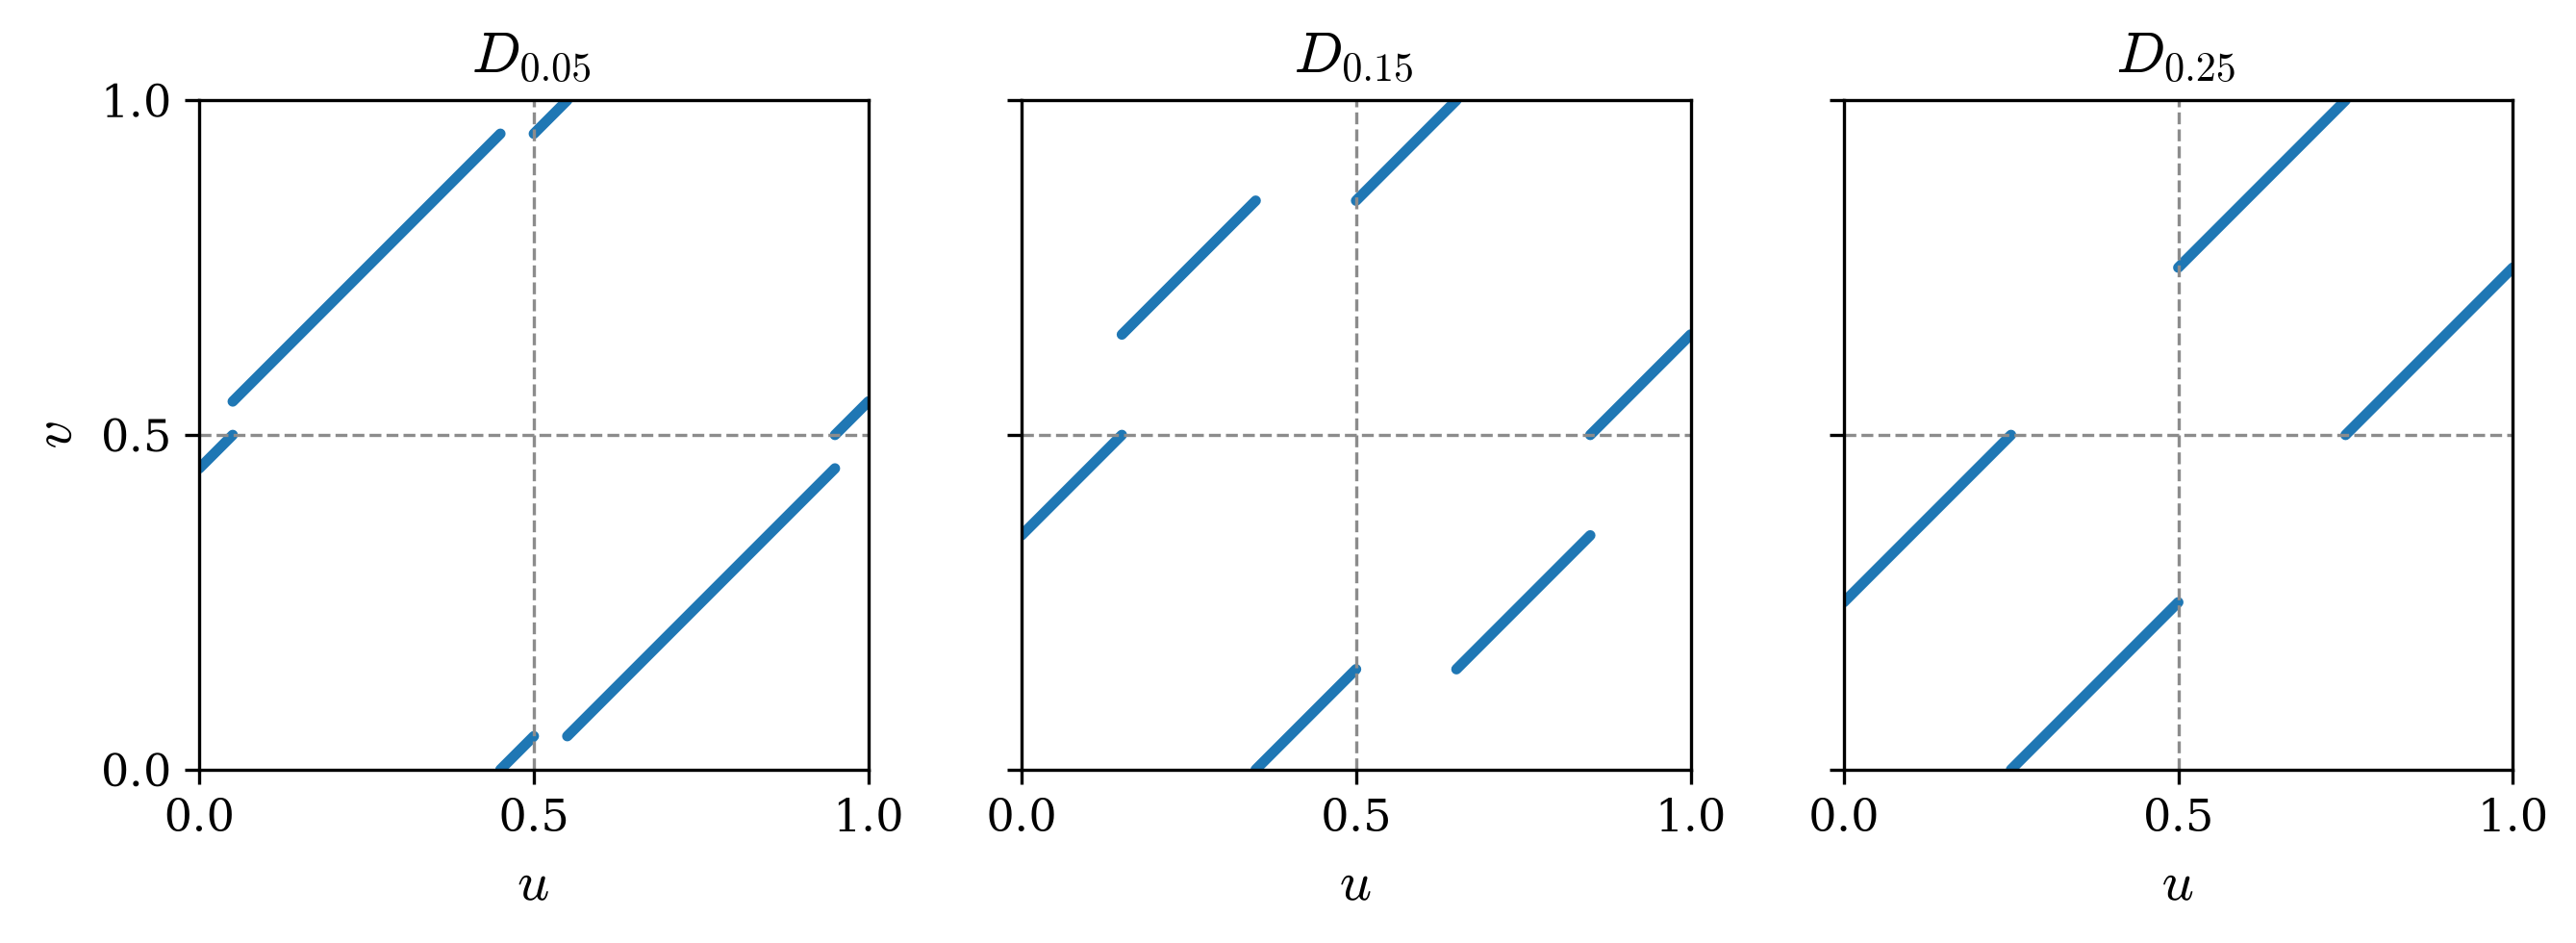
\includegraphics[width=0.95\textwidth]{images/D_seed_supports.png}
\caption{Supports of the upper seeds $D_q$ of Proposition~\ref{prop:upper-seed} for $q=0.05$, $0.15$ and $0.25$; dashed lines mark $u=\frac12$ and $v=\frac12$.
The copulas spread their mass uniformly on diagonal segments.
As $q$ increases, the four strips of width $q$ grow while the two strips of width $\frac12-2q$ shrink, degenerating at $q=\frac14$.
The family traces the upper edge of $\Om$ above the same boundary $\phi=L(\beta)$, with $(\tau,\phi,\beta)=(8q^2,12q^2-\frac12,8q-1)$.}
\label{fig:D-seeds}
\end{figure}
\begin{comment}
\begin{figure}[htbp!]
\centering
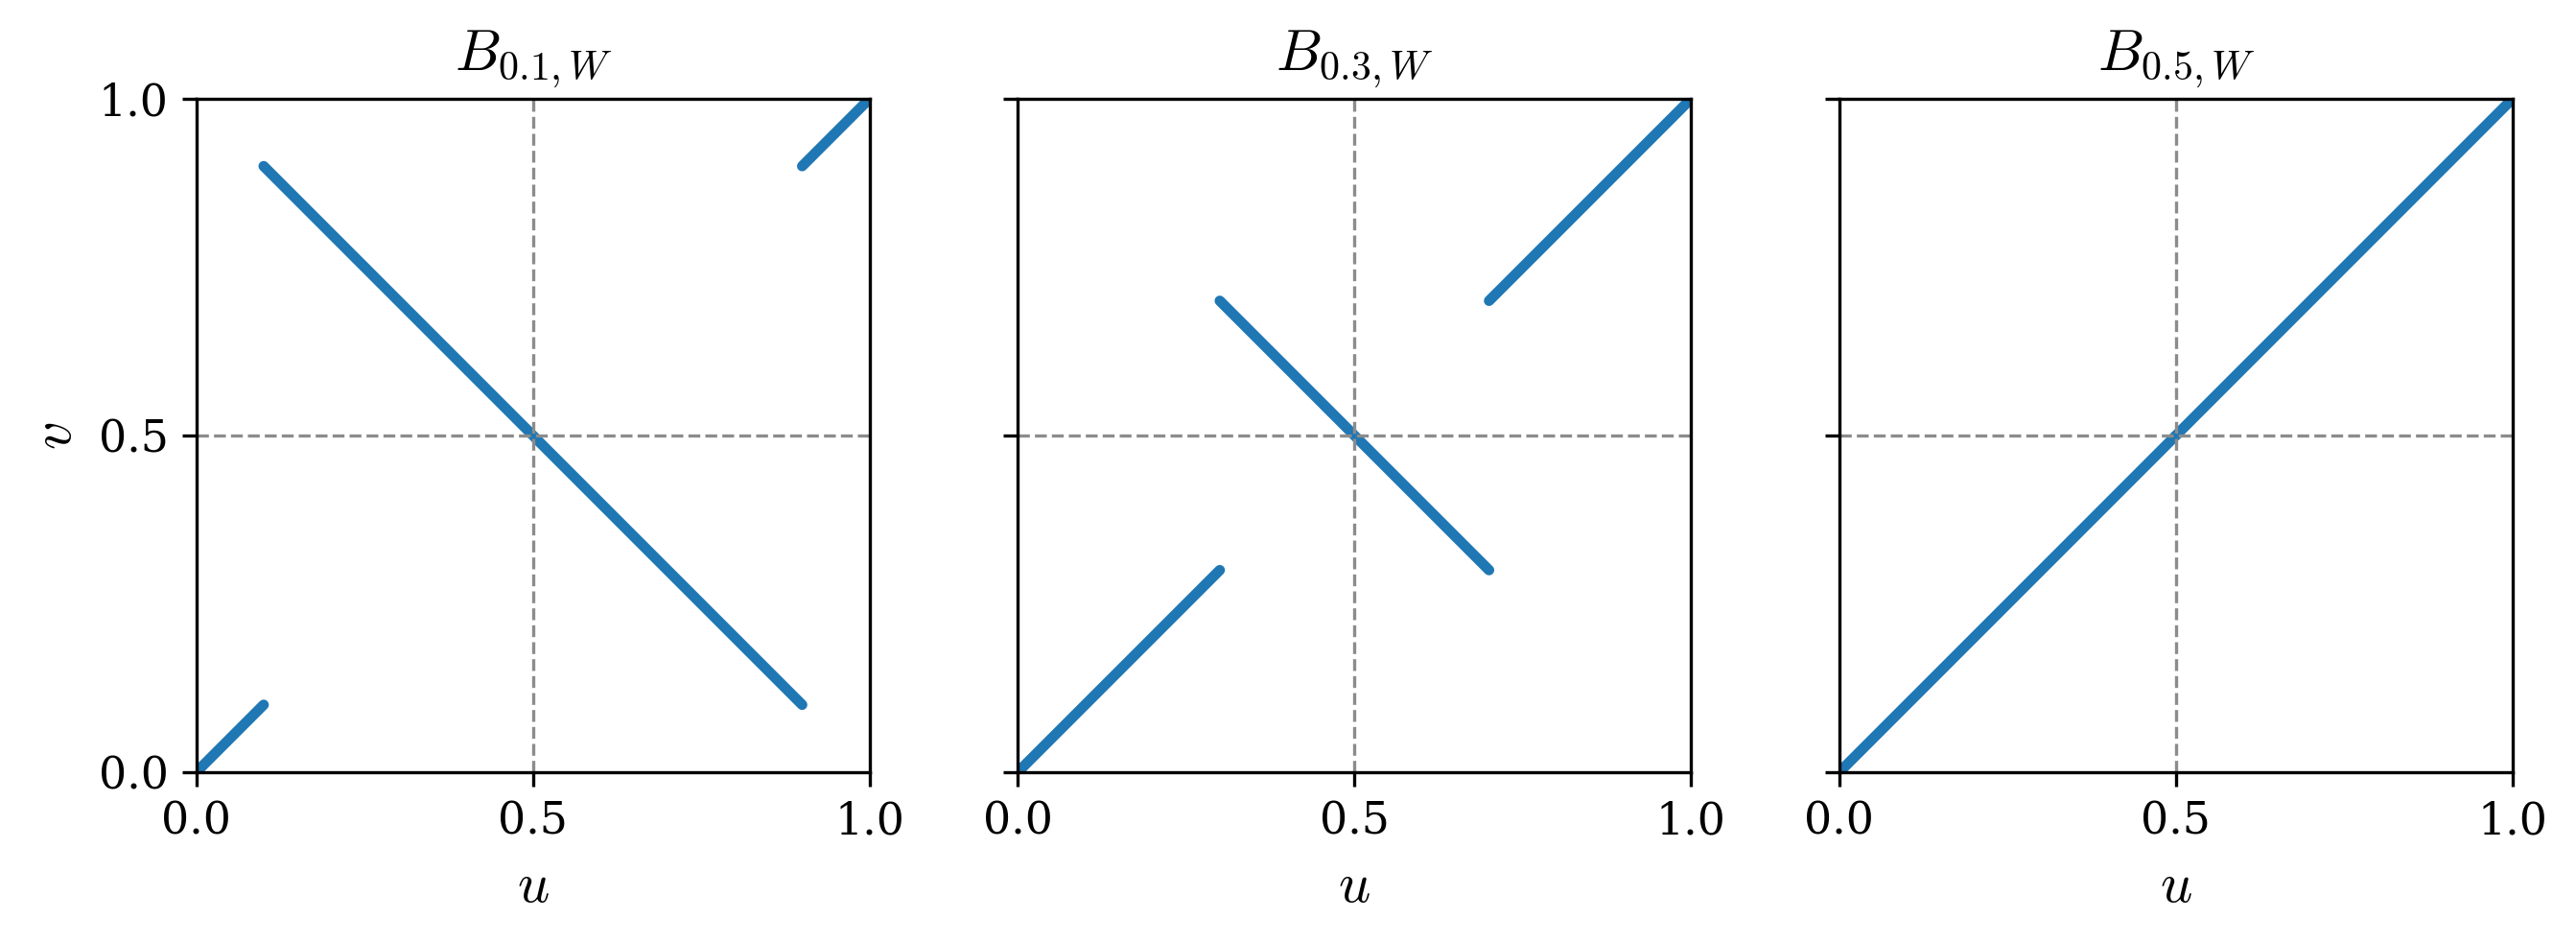
\includegraphics[width=0.95\textwidth]{images/B_aW_supports.png}
\caption{Supports of the ordinal sums $B_{a,W}$ of Remark~\ref{rem:boundary-edges} for $a=0.1$, $0.3$ and $0.5$; dashed lines mark $u=\frac12$ and $v=\frac12$.
The copulas coincide with $M$ outside the central square $[a,1-a]^2$, on which a rescaled copy of $W$ spreads its mass uniformly on the antidiagonal.
As $a$ increases, the central antidiagonal segment shrinks while the two diagonal segments grow, degenerating to $M$ at $a=\frac12$.
The family traces the edge $W$--$M$ of $\Om$ above the boundary $\phi=U(\beta)$, with $(\tau,\phi,\beta)=(1-2\alpha^2,1-\frac32\alpha^2,1-2\alpha)$ and $\alpha=1-2a$.}
\label{fig:BW-family}
\end{figure}

\begin{figure}[htbp!]
\centering
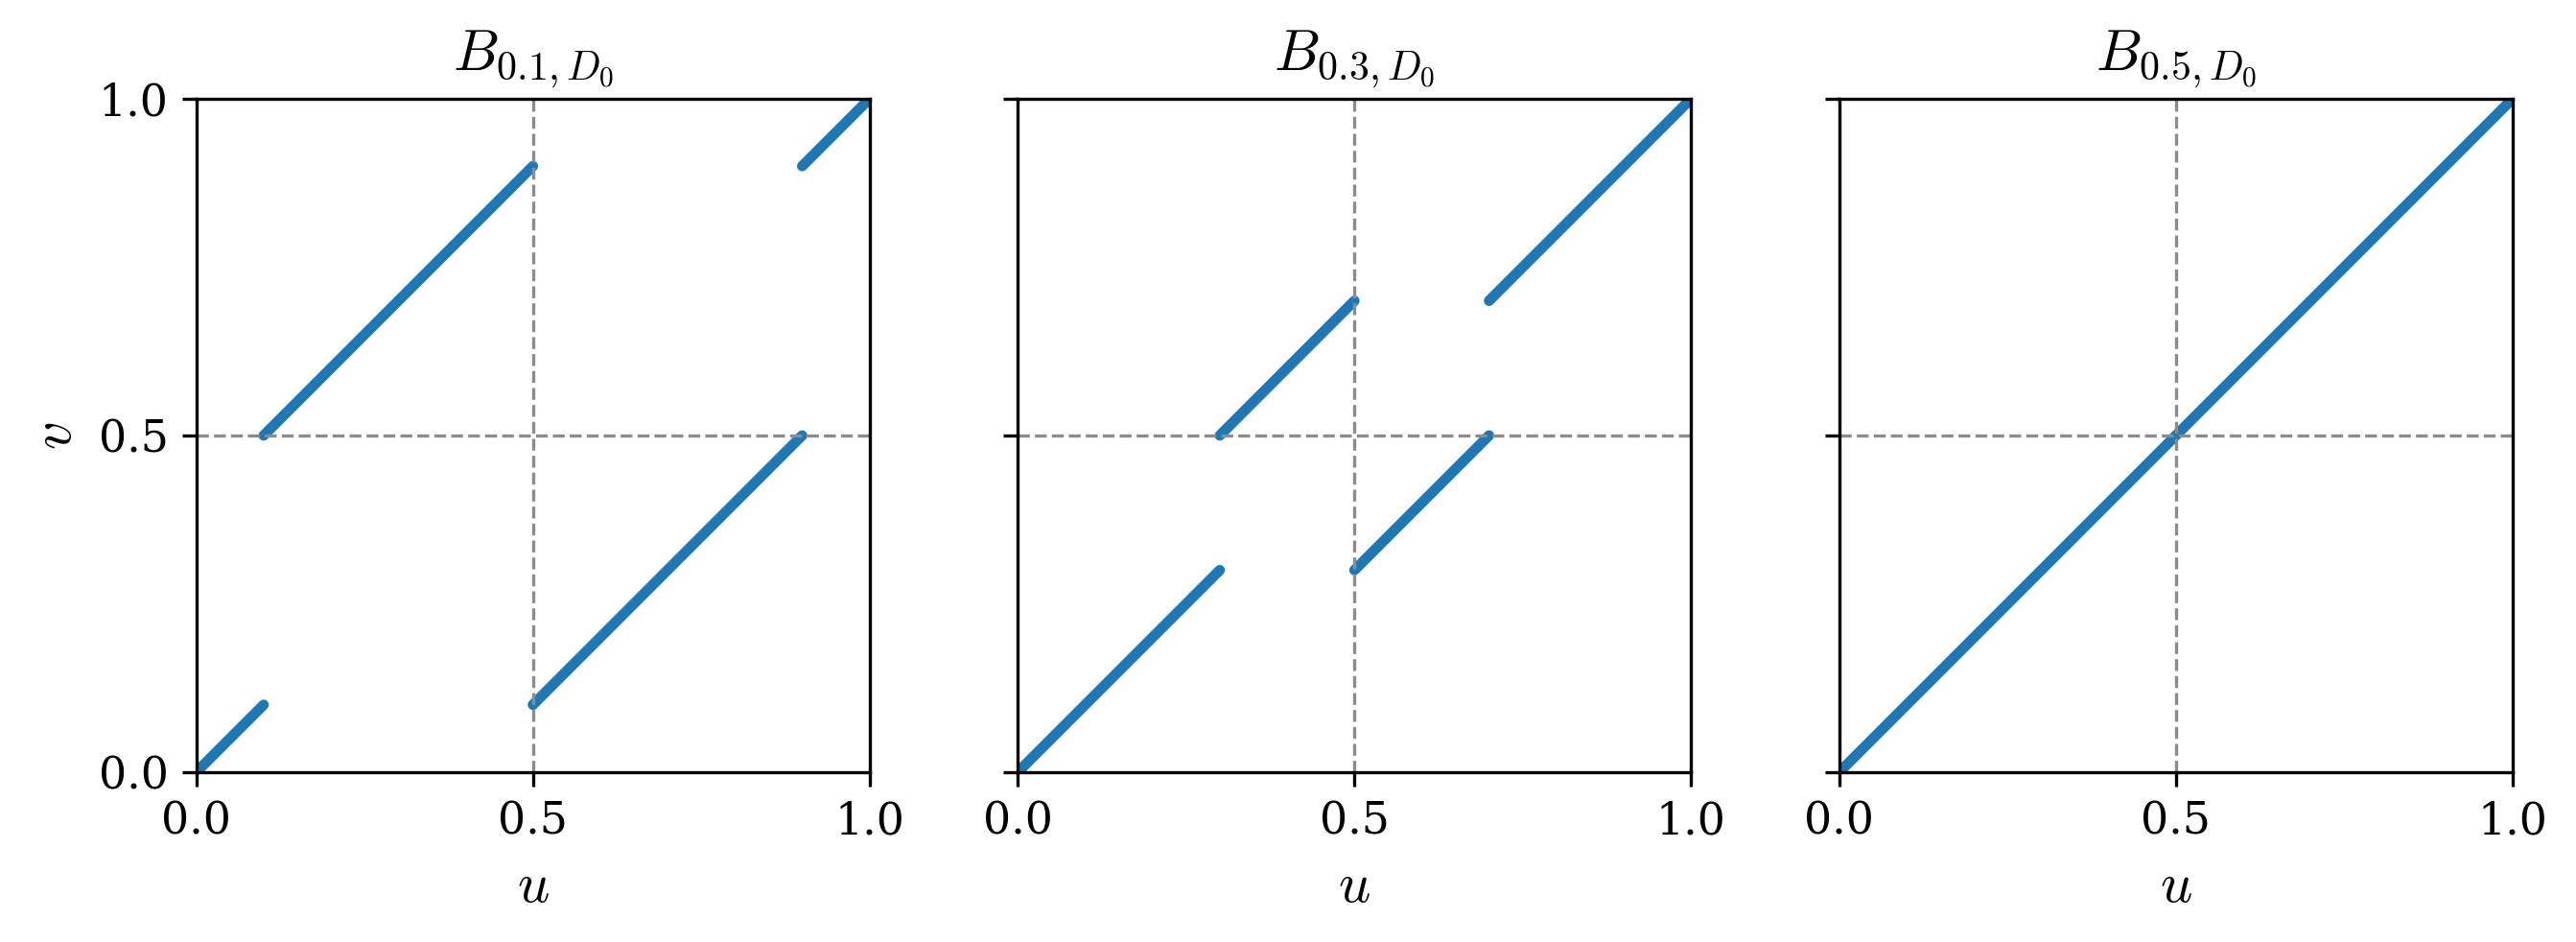
\includegraphics[width=0.95\textwidth]{images/B_aD0_supports.png}
\caption{Supports of the ordinal sums $B_{a,D_0}$ of Remark~\ref{rem:boundary-edges} for $a=0.1$, $0.3$ and $0.5$; dashed lines mark $u=\frac12$ and $v=\frac12$.
The copulas coincide with $M$ outside the central square $[a,1-a]^2$, on which a rescaled copy of $D_0$ spreads its mass uniformly on two parallel diagonal segments.
As $a$ increases, the two central segments shrink while the two corner segments grow, degenerating to $M$ at $a=\frac12$.
The family traces the edge $D_0$--$M$ of $\Om$ above the same boundary $\phi=U(\beta)$, with $(\tau,\phi,\beta)=(1-\alpha^2,1-\frac32\alpha^2,1-2\alpha)$ and $\alpha=1-2a$.}
\label{fig:BD0-family}
\end{figure}
\end{comment}
\begin{remark}[The four boundary edges]\label{rem:boundary-edges}
The seed families and their ordinal sums give explicit copulas for all four curved edges visible in Figure~\ref{fig:region}.
Indeed, let $\alpha\in[0,1]$ and $a=(1-\alpha)/2$.
Applying \eqref{eq:ordinal-sum} first to $W=A_0$ and then to $D_0$ gives
\begin{align*}
(\tau,\phi,\beta)(B_{a,W})
&=\bigl(1-2\alpha^2,\,1-\tfrac32\alpha^2,\,1-2\alpha\bigr),\\
(\tau,\phi,\beta)(B_{a,D_0})
&=\bigl(1-\alpha^2,\,1-\tfrac32\alpha^2,\,1-2\alpha\bigr).
\end{align*}
As $\alpha$ decreases from $1$ to $0$, the first family traces the edge from $W$ to $M$ and the second the edge from $D_0$ to $M$. %; their supports are shown in Figures~\ref{fig:BW-family} and~\ref{fig:BD0-family}.
Writing $b=1-2\alpha$, both lie above the upper boundary $p=U(b)$ of the $(\phi,\beta)$-region; the first satisfies $t=\ell(p)$ and the second $t=u(p)$.
Together with $A_r$, which traces the edge $W$--$A_{1/2}$, and $D_q$, which traces $D_0$--$D_{1/4}$ above $p=L(b)$, these families account for all four edges.
\end{remark}


\section{Proof of the main result}\label{sec:proof}

\begin{proof}[Proof of Theorem~\ref{thm:main}]
\emph{Necessity.}
If $(t,p,b)=(\tau(C),\phi(C),\beta(C))$ for some $C\in\C$, then $b\in[-1,1]$, and the constraints $L(b)\le p\le U(b)$ and $\ell(p)\le t\le u(p)$ hold by Proposition~\ref{prop:known}.

\emph{Sufficiency.}
Fix $b\in[-1,1]$, $p\in[L(b),U(b)]$ and $t\in[\ell(p),u(p)]$, and put $k\coloneqq 1-b\in[0,2]$.
We first construct copulas $C^-$ and $C^+$ with
\begin{equation}\label{eq:Cpm-goal}
\tau(C^-)=\ell(p),\qquad \tau(C^+)=u(p),\qquad \phi(C^\pm)=p,\qquad \beta(C^\pm)=b.
\end{equation}
Consider the function
\[
F_b(\alpha)\coloneqq 1-\tfrac34\alpha^2-\tfrac34 k\alpha+\tfrac{3}{16}k^2,
\qquad \alpha\in\bigl[\tfrac k2,1\bigr].
\]
Comparing with \eqref{eq:boundary-functions} gives
\[
F_b(\frac k2)=1-\frac38k^2=U(b),
\qquad F_b(1)=\frac14-\frac34k+\frac{3}{16}k^2=L(b).
\]
Moreover, $F_b'(\alpha)=-\frac32\alpha-\frac34 k<0$ except at the single endpoint $(k,\alpha)=(0,0)$.
Thus $F_b$ maps $[\frac k2,1]$ continuously onto $[L(b),U(b)]$, and there exists $\alpha\in[\frac k2,1]$ with $F_b(\alpha)=p$.
If $\alpha=0$, then $b=p=t=1$, so $M$ attains $(t,p,b)$ and the claim follows; hence assume $\alpha>0$ from now on.

Set $x\coloneqq 1-\frac k\alpha$; then $x\in[-1,1]$ because $\frac k2\le\alpha$, and $\alpha x+1-\alpha=1-k=b$.
Moreover, expanding $L(x)=\frac{3}{16}(2-\frac k\alpha)^2-\frac12$ yields
\begin{equation}\label{eq:scaling-identity}
\alpha^2L(x)+1-\alpha^2
=1-\tfrac34\alpha^2-\tfrac34 k\alpha+\tfrac{3}{16}k^2
=F_b(\alpha)=p.
\end{equation}
Let $P=A_{(x+1)/4}$ and $Q=D_{(x+1)/8}$ be the seed copulas of Propositions~\ref{prop:lower-seed} and~\ref{prop:upper-seed}, so that
\[
\bigl(\tau(P),\phi(P),\beta(P)\bigr)=\bigl(\ell(L(x)),L(x),x\bigr),
\qquad
\bigl(\tau(Q),\phi(Q),\beta(Q)\bigr)=\bigl(u(L(x)),L(x),x\bigr),
\]
and define $C^-\coloneqq B_{a,P}$ and $C^+\coloneqq B_{a,Q}$ with $a\coloneqq \frac{1-\alpha}{2}$.
By \eqref{eq:ordinal-sum} and \eqref{eq:scaling-identity}, $\beta(C^\pm)=\alpha x+1-\alpha=b$ and $\phi(C^\pm)=\alpha^2L(x)+1-\alpha^2=p$.
Since $\ell$ and $u$ are affine with $\ell(1)=u(1)=1$, they commute with the map $z\mapsto\alpha^2z+1-\alpha^2$.
Thus, by \eqref{eq:ordinal-sum},
\[
\tau(C^-)=\alpha^2\ell(L(x))+1-\alpha^2=\ell\bigl(\alpha^2L(x)+1-\alpha^2\bigr)=\ell(p),
\]
and likewise $\tau(C^+)=u(p)$; this proves \eqref{eq:Cpm-goal}.

Let $C_s\coloneqq (1-s)C^-+sC^+$ for $s\in[0,1]$, a copula by convexity of $\C$.
The functionals $\phi$ and $\beta$ are affine in the copula by \eqref{eq:phi-def} and \eqref{eq:beta-def}, so $\phi(C_s)=p$ and $\beta(C_s)=b$ for all $s$.
Since $\Q$ is symmetric and affine in each argument,
\[
\tau(C_s)=\Q(C_s,C_s)=(1-s)^2\,\tau(C^-)+2s(1-s)\,\Q(C^-,C^+)+s^2\,\tau(C^+)
\]
is a polynomial in $s$ with $\tau(C_0)=\ell(p)$ and $\tau(C_1)=u(p)$, and the intermediate value theorem yields $s\in[0,1]$ with $\tau(C_s)=t$.
Hence every point of the right-hand side of \eqref{eq:region} is attained, which completes the proof.
\end{proof}

\begin{corollary}[Convexity and fixed-footrule sections]\label{cor:fixed-phi}
The region $\Om$ is compact and convex.
For $p\in[-\frac12,1]$, define
\[
b_-(p)\coloneqq 1-\sqrt{\tfrac83(1-p)},\qquad
b_+(p)\coloneqq \min\Bigl\{1,-1+\tfrac4{\sqrt3}\sqrt{p+\tfrac12}\Bigr\}.
\]
Then the section of $\Om$ at fixed footrule $p$ is the possibly degenerate rectangle
\begin{equation}\label{eq:fixed-phi-section}
\bigl\{(t,b)\in\R^2:(t,p,b)\in\Om\bigr\}
=[\ell(p),u(p)]\times[b_-(p),b_+(p)].
\end{equation}
Thus, once the value of Spearman's footrule is fixed, the admissible values of Kendall's tau and Blomqvist's beta vary independently over their respective intervals.
\end{corollary}

\begin{proof}
By Theorem~\ref{thm:main}, the region $\Om$ is closed and bounded, hence compact.
The function $L$ is convex, the function $U$ is concave, and $\ell$ and $u$ are affine.
Hence the bounds on $b$, the epigraph of $L$, the hypograph of $U$ and the two affine bounds on $t$ are convex sets, so their intersection $\Om$ is convex.

Now fix $p\in[-\frac12,1]$.
Since $1+b\ge0$ and $1-b\ge0$ for $b\in[-1,1]$, solving $L(b)\le p\le U(b)$ for $b$ gives
\[
1-\sqrt{\tfrac83(1-p)}\le b
\le \min\Bigl\{1,-1+\tfrac4{\sqrt3}\sqrt{p+\tfrac12}\Bigr\}.
\]
The bounds $\ell(p)\le t\le u(p)$ do not involve $b$, which proves \eqref{eq:fixed-phi-section}.
\end{proof}

\begin{corollary}[Exact $(\tau,\beta)$-region]\label{cor:beta-tau}
We have
\[
\bigl\{(\tau(C),\beta(C)):C\in\C\bigr\}
=\Bigl\{(t,b)\in[-1,1]^2:\ \tfrac14(1+b)^2-1\le t\le 1-\tfrac14(1-b)^2\Bigr\},
\]
recovering the region stated in \cite[Exer.~5.17]{nelsen2006introduction} and obtained in \cite[Thm.~5 and Cor.~6]{kokolbukovsek2019relation}.
\end{corollary}

\begin{proof}
By Theorem~\ref{thm:main}, the projection of $\Om$ onto the $(t,b)$-coordinates has, over each fixed $b\in[-1,1]$, the fibre
\(
\bigcup_{p\in[L(b),U(b)]}[\ell(p),u(p)]
\),
which is the projection onto the $t$-axis of the set
\[
S_b\coloneqq
\bigl\{(p,t)\in\R^2:\ L(b)\le p\le U(b),\ \ell(p)\le t\le u(p)\bigr\}.
\]
Since $\ell$ and $u$ are affine and $L(b)\le U(b)$, the set $S_b$ is convex, so its projection onto the $t$-axis is an interval.
Because $\ell$ and $u$ are increasing, the left endpoint is $\ell(L(b))$ and the right endpoint is $u(U(b))$.
Evaluating with \eqref{eq:boundary-functions} gives
\[
\ell(L(b))=\frac14(1+b)^2-1,\qquad
u(U(b))=1-\frac14(1-b)^2,
\]
which proves the claim.
\end{proof}

\begin{remark}\label{rem:fibre}
The spread $u(p)-\ell(p)=\frac23(1-p)$ of admissible values of $\tau$ over an admissible pair $(\phi,\beta)=(p,b)$ depends on $p$ alone, so fixing $\beta$ narrows the range of $\tau$ no further than the $(\tau,\phi)$-bounds \eqref{eq:ft-region} already do.
More precisely,
\[
\ell(p)=p-\frac{1-p}{3},\qquad
u(p)=p+\frac{1-p}{3},
\]
so every such fibre is symmetric about $t=p$.
In particular, for every admissible pair $(p,b)$ there exists a copula $C$ satisfying
\[
\tau(C)=\phi(C)=p,\qquad \beta(C)=b.
\]
Equivalently, $\Om$ is invariant under the affine involution $(t,p,b)\mapsto(2p-t,p,b)$.
This is a geometric symmetry of the attainable region; the argument does not identify a canonical operation on copulas that induces the involution.
In this attainable-region sense, Blomqvist's beta adds no sharp restriction on Kendall's tau once Spearman's footrule is known.
This complements the similarity-measure computations in \cite[Sec.~5]{kokolbukovsek2023exact}, by which knowing $\beta$ alone already conveys, on average, very little information about the possible values of $\tau$.
\end{remark}

\section{Concluding remarks}\label{sec:conclusion}

For fixed $b\in[-1,1]$, the area of the section of $\Om$ in the $(t,p)$-coordinates is
\[
A(b)
\coloneqq \int_{L(b)}^{U(b)}\bigl(u(p)-\ell(p)\bigr)\de p
=\frac23\int_{L(b)}^{U(b)}(1-p)\de p
  =\frac{3}{256}(3-b)^2(1+b)(5-3b).
\]
Differentiating gives
\[
A'(b)=\frac{3}{64}(3-b)\bigl(3(b-1)^2-4\bigr).
\]
At $b=-1$ the section degenerates to a line segment, while the sign of $A'$ shows that $A$ has the unique maximum $\frac14+\frac{\sqrt3}{6}$ at $b=1-\frac{2}{\sqrt3}$.
Integrating these sectional areas gives the volume of the region,
\[
\operatorname{vol}(\Om)
=\int_{-1}^{1}A(b)\de b
=\frac{3}{256}\int_{-1}^{1}
\bigl(-3b^4+20b^3-34b^2-12b+45\bigr)\de b
=\frac{31}{40},
\]
which is $\frac{31}{240}\approx0.129$ of the volume of the bounding box $[-1,1]\times[-\frac12,1]\times[-1,1]$.
For comparison, $\operatorname{vol}(\Omega_{\phi,\gamma,\tau})=\frac{3}{16}$ and $\operatorname{vol}(\Omega_{\beta,\phi,\gamma})=\frac{19}{40}$, see \cite{kokolbukovsek2026footrule,kokolbukovsek2026exact}.
This relatively large volume reflects Remark~\ref{rem:fibre}: the three coefficients $\tau$, $\phi$ and $\beta$ constrain one another only through the two bivariate regions.

In view of \cite{kokolbukovsek2026exact,kokolbukovsek2026footrule} and Theorem~\ref{thm:main}, the next natural problems are the exact region $\Omega_{\beta,\gamma,\tau}$ and the full four-dimensional region determined by $\beta$, $\phi$, $\gamma$ and $\tau$.
To the best of our knowledge, both remain open.
Exact regions involving Spearman's rho also appear to be considerably harder; cf.~\cite{schreyer2017exact,kokolbukovsek2024rhofootrule,tschimpke2025revisiting}.

\bibliographystyle{plainnat}
\bibliography{references}

\end{document}

